\chapter{Uncertainty quantification in parameter identification}
\label{UQ}
Uncertainty quantification (UQ) aims at taking into account the uncertainties in the parameters of the model of a physical system and at studying their impact onto the system response. A well-established representation of an uncertainty quantification problem is presented next. The rationale is that any such problem can be represented by a combination of these elements, as sketched in \cref{fig: UQ_steps}:
\begin{itemize}
    \item Definition of the computational model $\mathcal{M}$ of the physical system. This is rather broad step that may refer to an analytical function in its simplest form, or an black box containing different levels of partial differential equations (e.g., finite element packages or finite difference packages). In general, the computational model $\mathcal{M}$ maps a set of input parameters $\boldsymbol{x})$ to one or more \acrfull{QoI}. often referred to as \textit{model responses}.
    \item The sources of uncertainties in input space. This steps entails the identification of the input parameters that are uncertain and their description within a probabilistic context.
    \item Uncertainty propagation from input parameters $\boldsymbol{x}$ to $\boldsymbol{y}$. This step refers to the quantification of the uncertainty in the \acrshort{QoI} by propagating the uncertainty of the input space through the computational model $\mathcal{M}$. 
    \item Iterative updating of the source of uncertainty. This step may refer to several techniques used to updated the information available on the sources of uncertainty identified above. Examples includes \textit{sensitivity analysis} or \textit{Bayesian inference}. If we are using \textit{sensitivity analysis} to update the uncertainties, it can be explicitly called as \textit{forward problems}. If we are using \textit{Bayesian inference} to update the uncertainties, it can be called as \textit{inverse problems}.
\end{itemize}
\begin{figure}[htbp]
    \centering
    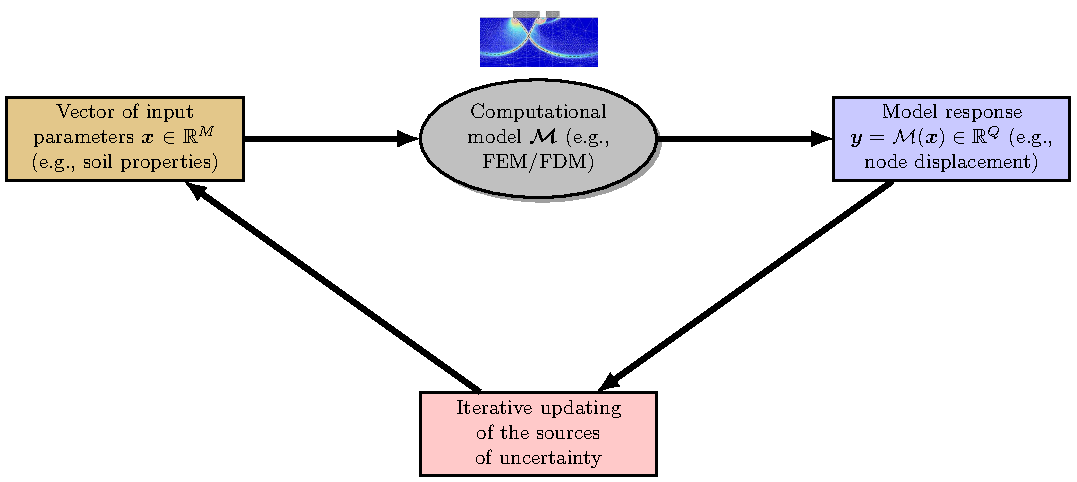
\includegraphics[width = 140mm]{Figures/figure-UQ_steps.pdf}
    \caption{Global framework for uncertainty quantification}
    \label{fig: UQ_steps}
\end{figure}

\section{Problem statement in UQ}
Modern engineering applications simulate UQ depending on a large number of input parameters. And the computational model is often treated as black box, i.e., only the input parameters $\boldsymbol{x}$ and model response $\boldsymbol{y}$ are available. Dealing with uncertainties using \textit{Monte Carlo} in such systems poses a major challenge to computational resources. In such cases, the underlying model can be substituted by a surrogate $\tilde{\mathcal{M}}$ as shown in \cref{fig: UQ_surrogate}. The solid line denotes the current working flow. Surrogate models enable many forward and inverse UQ analyses on high-fidelity computational models, by approximating the original model with a cheap-to-evaluate replacement model. In high dimensions, however, the performance of surrogate models decreases, while the cost of computing and storing them increases. This is well-known issue as the \textit{curse of dimensionality}. Therefore, there is never enough data for constructing a perfect surrogate in high dimensions. To alleviate this, we can perform \textit{experiment of design} sequentially using \textit{active learning} techniques or choose an appropriate type of surrogates. Next, we will introduce these in the next sections.

\begin{figure}[htbp]
    \centering
    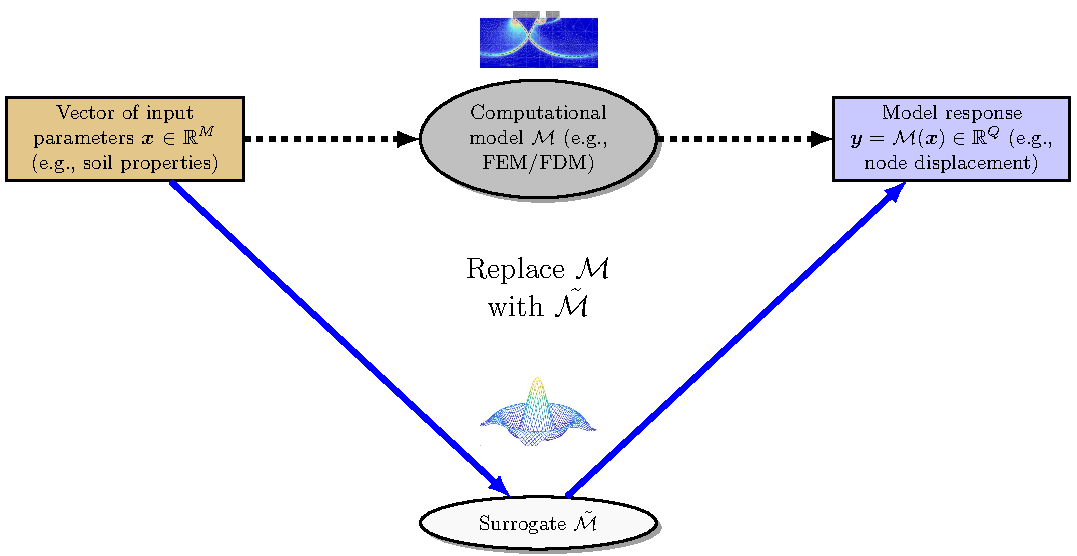
\includegraphics[width = 140mm]{Figures/figure-UQ_surrogate.pdf}
    \caption{Using a surrogate to obtain the model response}
    \label{fig: UQ_surrogate}
\end{figure}

\section{Surrogate model}

Computer modelling is used in nearly every field of science and engineering. Often, these computer codes model complex phenomena, have many input parameters,
and are expensive to evaluate. In order to explore the behavior of the model under uncertainty (e.g., uncertainty propagation, parameter calibration from data or sensitivity analysis), many
model runs are required. However, if the model is costly, only a few model evaluations can be afforded, which often do not suffice for thorough uncertainty quantification. In engineering and applied sciences, a popular work-around in this situation is to construct a reduced-order surrogate model. A reduced-order surrogate model is a cheap-to-evaluate proxy of the original model, which typically can be constructed from a relatively small number of model evaluations and approximates
the input-output relation of the original model well. Since the surrogate model is cheap to evaluate, uncertainty quantification can be performed at a low cost by using the surrogate
model instead of the original model. Therefore, surrogate modelling aims at constructing a metamodel that provides an accurate approximation to the original model while requiring as few model evaluations as possible for its construction. A surrogate model $\tilde{\mathcal{M}}$ can be expressed as:
\begin{equation}
\label{eq:surrogate_model}
    \tilde{\mathcal{M}}(\boldsymbol{X})  \overset{\mathrm{def}}{=} \mathcal{M}(\boldsymbol{X}) - \mathcal{R}(\boldsymbol{X})
\end{equation}
\begin{equation}
\label{eq:surrogate_model}
    \tilde{\mathcal{M}}(\boldsymbol{X})  \overset{\mathrm{def}}{=} \mathcal{M}(\boldsymbol{X}) - \mathcal{R}(\boldsymbol{X})
\end{equation}
where $\mathcal{R}$ is the residual between the original model and the surrogate.




The general concept of \cref{eq:surrogate_model} is straightforward: given a finite set of input realisations and their corresponding model output, known as \textit{experiment of design}. A variety of methods is available in the surrogate modelling, in which some of them are listed in the \cref{table: All_Surrogates}.


\begin{table}[htbp]
\caption{Surrogate model choices}
\label{table: All_Surrogates}
\begin{tabular}{lll}
\hline
Name                              & \multicolumn{1}{c}{Shape} & \multicolumn{1}{c}{Parameters} \\ \hline
Polynomial chaos expansions       &                           $\tilde{\mathcal{M}}(\boldsymbol{x})
=
\sum_{\boldsymbol{\alpha} \in \mathcal{A} } 
c_{\alpha} \Psi_{\alpha} (\boldsymbol{x})$&                                $c_{\alpha}$\\
Low-rank tensor approximations    &                           $\tilde{\mathcal{M}}(\boldsymbol{x})
=
\sum_{l=1}^{R} b_{l}
\left ( 
\prod_{i=1}^{M}  v_{l}^{i}x_{i}
 \right ) 
$&                                $b_{l}, \  z_{k,l}^{i}$\\
Kriging (a.k.a Gaussian processs) &                           $\tilde{\mathcal{M}}(\boldsymbol{x})
=
\boldsymbol{\beta}^{T} \cdot \boldsymbol{f}(\boldsymbol{x})
 + Z(\boldsymbol{x},\omega)$&                                $\boldsymbol{\beta}, \ \sigma_{Z}^{2}, \  \boldsymbol{\theta}$\\
Support vector machines           &                           $\tilde{\mathcal{M}}(\boldsymbol{x})
=
\sum_{i=1}^{m}
a_{i} K(\boldsymbol{x}_{i},\boldsymbol{x}) 
+b$&                                $\boldsymbol{a}, \ b$\\
Neural networks                   &                           $\tilde{\mathcal{M}}(\boldsymbol{x})
=
f_{n}\left ( 
\cdots f_{2}(
b_{2} + f_{1}(
b_{1} + \boldsymbol{w}_{1} \cdot \boldsymbol{x}
)
\cdot \boldsymbol{w}_{2}
)
\right ) $&                                $\boldsymbol{w}, \ \boldsymbol{b}$\\ \hline
\end{tabular}
\end{table}
Why not neural networks?

Model reduction lets us create approximate models that are fast to solve, and — importantly — it provides us a rigorous mathematical basis on which to establish strong guarantees of accuracy of the low-dimensional model. This is in contrast with black-box machine learning methods (ANN), where we just have to hope that our training data was rich enough to yield a sufficiently accurate surrogate model. This is especially problematic for engineering applications where we often need to issue extrapolatory predictions.

\subsection{Polynomial chaos expansion}
Metamodelling (or surrogate modelling) attempts to offset the increased costs of stochastic modelling by substituting the expensive-to-evaluate computational models (e.g. finite element models, FEM) with inexpensive-to-evaluate surrogates.
Polynomial chaos expansions (PCE) are a powerful metamodelling technique that aims at providing a functional approxmation of a computational model through its spectral representation on a suitably built basis of polynomial functions.

Different from other surrogate modelling approaches such as support vector machine, Gaussian process regression, or neural networks, the mathematical theory underlying reduced-order models can lead to more reliable and robust predictive capability \citep{frangos2010,kapteyn2021}.

Different from Monte Carlo simulation (MCS) which is based on point-to-point exploring the output space, PCE assumes a generic structure, which better exploits the available runs of the FE realizations.

\section{Data-driven inference}
\subsection{Inference of the marginal distributions}
\subsection{Inference of the copula}
\section{Dimensionality reduction}


Engineering problems inherently involve high dimensionality, posing challenges for learning methods like surrogate modeling. Technical constraints impact the storage and processing of such huge amount of data. Furthermore, as input and output data expand, independent scalar surrogate models show inadequate in accurately capturing the covariance matrix of the original data, leading to less reliable predictions. Consequently, in high dimensional space, the need for dimensionality reduction technique (DR) becomes more critical. 


\subsection{Linear DR technique}

\subsection{Nonlinear DR technique}

\section{DR-based surrogate modelling}

\section{Inverse problems in UQ}

When faced with large-scale forward models characteristic of many engineering and science applications, high computational cost arises from: (1) In the large-scale setting, performing thousands or millions of forward simulations is often computationally intractable; (2)  the dimension of the input space are complex; (3) sampling may be complicated by the large dimensionality of the input space. Thus, to reduce the computational cost of solving of a statistical inverse problem, methods can be broadly in three groups: (1) Surrogate models to accelerate a forward simulation; (2) Reduce the dimension of the input space,i.e., sensitive analysis; (3) Efficient sampling method to posterior,i.e., MCMC.



\subsection{Inverse problems}

\subsection{Bayesian inference}

\subsection{Bayesian calibration}

\subsection{Sampling methods}

\subsubsection{Using the CDF}



\subsubsection{Rejection sampling}


\subsubsection{Importance sampling}

Often, in practical Bayesian models, it is not possible to obtain samples directly from p.x j y1WT / due to its complicated functional form.

\subsubsection{Sequential Monte Carlo}


\subsubsection{Markov chain Monte Carlo}



\subsection{Choice of sampling method}


\subsection{Seqential Bayesian inference}


\section{Sequential enrichment for surrogate model}

Traditional large-scale physics-based models are intractable to solve real-time, many-query context problem. 


Instead of sampling the whole experimental design at once, it has been proposed to use sequential enrichment. Starting with
a small experimental design, additional points are chosen based on the last computed sparse
solution. In the context of machine learning, sequential sampling is also known as active learning.  In all cases, numerical examples show that the sequential strategy generally leads to solutions with
a smaller validation error compared to non-sequential strategies

\section{Sensitivity analysis}



\section{Uncertainty quantification in high dimensions}
\subsection{Forward problem}

Some Monte Carlo methods, including rejection sampling, importance sampling and particle filtering. The trouble with these methods is that they do not work well in high
dimensional spaces. The most popular method for sampling from high-dimensional distributions
is Markov chain Monte Carlo or MCMC.
\subsection{High dimensional problem}

Some Monte Carlo methods, including rejection sampling, importance sampling and particle filtering. The trouble with these methods is that they do not work well in high
dimensional spaces. The most popular method for sampling from high-dimensional distributions
is Markov chain Monte Carlo or MCMC.


\subsection{Choice for sampling method in high dimensions}